% !TEX root = Thesis.tex

%==============================================================================
\chapter{Raman manipulation between spin-momentum state components}
\label{chap:raman_manipulation}
%==============================================================================

After the theoretical description of the Raman processes occurring in the diffraction of ultracold atomic ensembles, the following step consists in the manipulation of momentum and spin states components. The process has a strong resemblance with the previously described, with the added factor that now every momentum state also carries a different internal energy state. This is due to Raman transitions taking place between Zeeman levels that the ground state of erbium was split into. For the experimental process to function as expected, it is required a given magnetic field $\vec{B}_\text{R} = B_{\text{R}} \vec{e}_x$ along the optical beams axis $x$. This field will produce the Zeeman splitting of the ground state, and the Raman beams will be in charge of producing the transitions, separating the atomic ensemble into multiple energy levels. However, the two photon detuning condition must be fulfilled for this process to happen, and now it corresponds with the energy difference between two Zeeman split states $\Delta E_\text{R} = g_J \mu_B B_\text{R}$ \cite{Foot2005}. Due to this, knowing the exact value of $\Delta E_\text{R}$ becomes a key factor, and any background magnetic fields affecting the \ac{bec} can produce non-desired mixed transitions in the energetic scheme. For this reason, a preparatory experiment must be carried out, that allows the estimation of $\Delta E_\text{R}$ and helps with the compensation of background fields in favour of the known $\vec{B}_\text{R}$ field.

\section{\Acl{rf} transitions and the Stern-Gerlach experiment}\label{sec:rf_transitions}

The objective of this experiment is to quantify the Zeeman splitting induced into an erbium \ac{bec}. As it can be seen in Figure \ref{fig:erbium_scheme}, the energetic ground state of erbium has a total electronic angular momentum of $J = 6$. When the atomic ensemble is being affect by a magnetic field $\vec{B}_\text{H}$, the ground state gets Zeeman split into $2J+1 = 13$ energy states with the secondary quantum number $m_J = \text{-6, -5, ..., +6}$, each state with energy
\begin{equation}
	E_\text{Ze} = g_J \mu_B m_J B_\text{H},
\end{equation}
where $g_J$ represents the Landé g-factor and for this case it is $g_J\approx1.166$ \cite{Foot2005}. Due to the way in which the experimental set-up is constructed, the \ac{mot}'s \SI{583}{\nano\meter} beam light that interacts with erbium in the $z$ axis, by pushing the atoms against gravity, is $\sigma^-$ polarized \cite{Ulitzsch2016}. Due to the fact that this beam interacts mostly with the atomic ensemble, it pumps atoms into the energetic state with $m_J = -6$. Therefore, the atomic ensemble becomes spin polarized. To allow for transitions between these different Zeeman states, the atomic ensemble must interact with a \acf{rf} pulse. Moreover, in order to distinguish which spin states the \ac{rf}-pulse has transitioned the atomic ensemble into, a Stern-Gerlach experiment must be performed. This consists in the use of an inhomogeneous magnetic field $B_\text{IH}(\vec{r})$ that separates the atomic \ac{bec} spatially according the quantum number $m_J$. The force that allows this is commonly called Stern-Gerlach force and is due to the non-zero gradient applied to the Zeeman term in the hamiltonian \cite{Foot2005}
\begin{equation}
	\vec{F}_\text{SG}(\vec{r}) = \grad{(\vec{\mu}\cdot\vec{B}_\text{IH}(\vec{r}))},
\end{equation}
where $\vec{\mu}$ represents the atomic magnetic moment. Therefore, for $B_\text{IH}(\vec{r})$ pointing in any arbitrary $z$ direction, the force applied to the different $2J+1$ levels can be obtained as
\begin{equation}\label{eq:Stern-Gerlach_force}
	\vec{F}_\text{SG}(\vec{r}) = - g_J \mu_B m_J \frac{\partial B_\text{IH}(\vec{r})}{\partial z},
\end{equation}
which is $m_J$ dependant and produces, as a result, different contributions to the energetic states. This force will make possible the separation of a \ac{bec} in Zeeman orders after a given \ac{tof}. The use of \ac{rf}-transitions together with this SG-force permits the creation of an experimental set-up that can quantify the energetic difference between neighbouring Zeeman orders
\begin{equation}\label{eq:Zeeman_splitting_difference}
\Delta E_\text{Ze} = g_J \mu_B B_\text{H}.
\end{equation}

For a given spatially homogeneous field $\vec{B}_\text{H}$, interacting initially with an atomic ensemble. The experimental procedure can be described as follows:
\begin{itemize}
	\item \SI{2}{\milli\second} after the evaporation phase end, the \ac{rf}-pulse is applied while $\vec{B}_\text{H}$ is kept unchanged. This \ac{rf}-pulse has a given duration $t_\text{RF}$, an intensity $I_\text{RF}$ and a frequency $\nu_\text{RF}$. As a result, the transition between the initial state $m_J=-6$ to $m_J=-5\text{, ..., +6}$, is driven leading to population transfer if $\nu_\text{RF}\approx\frac{\Delta E_\text{Ze}}{\hbar}$ the resonant frequency for the Zeeman transition. Moreover, due to the fact that these transitions also result in Rabi oscillations, the magnitudes $t_\text{RF}$ and $I_\text{RF}$ must be adjusted to produce $\frac{\pi}{2}$ pulses and favour the population transference into the rest of Zeeman states.
	\item After the \ac{bec} interaction with the \ac{rf}-pulse, the ensemble falls due to gravity during a \acl{tof} $t_\text{TOF}$. In this time period, the magnetic field gradient $B_\text{IH}(\vec{r})$ is activated and the atomic \ac{bec} receives a state dependant Stern-Gerlach force given by Equation \eqref{eq:Stern-Gerlach_force}. This results in the spacial separation of the Zeeman levels after the \ac{tof}, which can be imaged by the absorption imaging phase.
\end{itemize}

As a result, the experiment allows to measure the resulting orders after a \ac{rf}-\ac{bec} interaction. By varying $\nu_\text{RF}$, one can make a measurement of the resonant frequency to the Zeeman splitting produced by any homogeneous field $\vec{B}_\text{H}$. In addition to the transition's line-width estimation, which is a parameter deeply related to the stability of $\vec{B}_\text{H}$ during the interaction time $t_\text{RF}$. To conclude, the experiment allows to measure the Zeeman splitting of any given field $\vec{B}_\text{H}$ and compensate for the effect that produces by adjusting the offset coils inside the vacuum chamber. This adjust the field to a value that reduces to the minimum  $\Delta E_\text{Ze}\approx0$. After this, a known field in the desired Raman beams $x$ direction can be added to the system. By repeating now the same \ac{rf} measurement, one obtains a fairly good estimation of the Zeeman splitting produced by the known field in the $x$ direction $\Delta E_\text{R}$. This value will give the two photon detuning condition for Raman manipulation in the following section. For a broader description of the procedure and experimental set-up refer to \cite{Ulitzsch2016}.

\section{Raman transitions between spin-momentum state components}\label{sec:raman_manipulation_theory}

Once the previous experiment has allowed to characterize the magnetic field $\vec{B}_{\text{R}}$ along the quantization axis $x$, Raman transitions between the Zeeman split states generated by $\vec{B}_{\text{R}}$ can be obtained with the use of two counter-propagating beams. As can be seen in Figure \ref{fig:raman_manipulation}, the optical set-up is very similar to the previous case. The two main differences are the addition of a magnetic field $\vec{B}_\text{R}$ along the Raman beams $x$ axis, and the change from linear to circular $\sigma^\pm$ polarization in the optical beams. As a result, now the 2$N$-photon Raman transitions generate orders that not only have different momentum components but also different spin values, in this case $m_J = \text{-6, -4, -2, 0, +2, +4, +6}$.

\begin{figure}[!htbp]\centering
	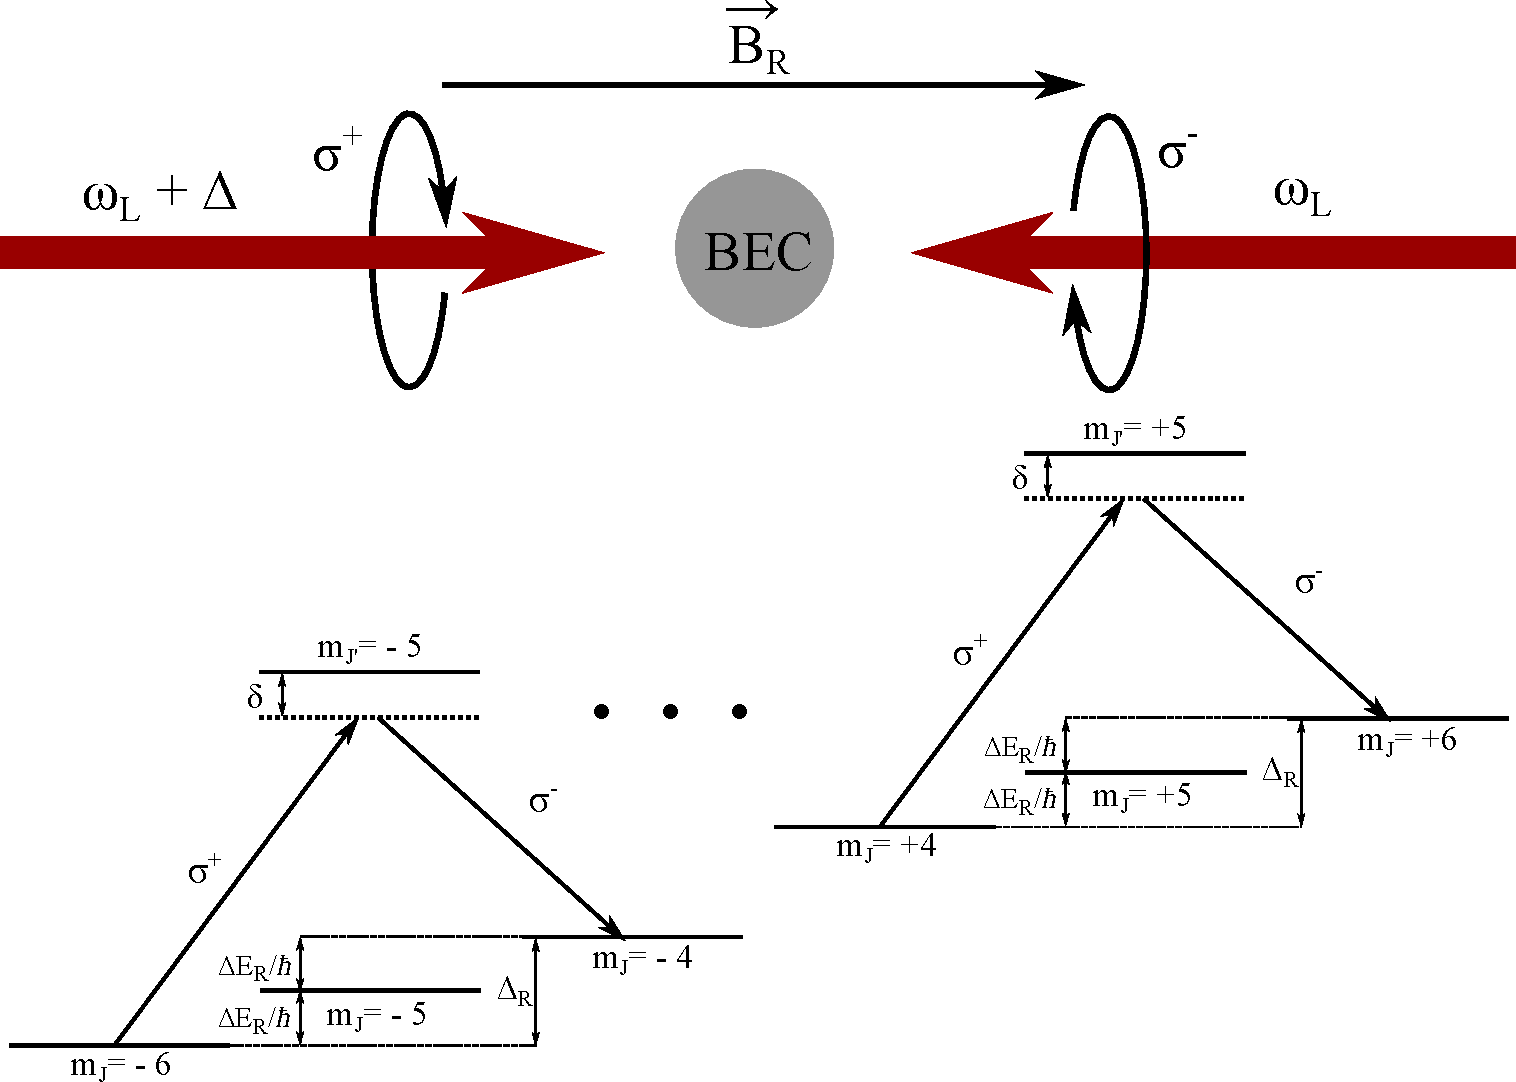
\includegraphics[width=0.9\columnwidth]{rama_spin_mainpulation_2.pdf}
	\caption[Experimental and energetic scheme of the 2$N$-photon Raman transition process in the spin-momentum configuration]{Experimental and energetic scheme of the 2$N$-photon Raman transition process in the spin-momentum configuration. In this case, the optical scheme is very similar to the described in Chapter \ref{chap:one_dimensional_lattices} with the addition of a magnetic field $\vec{B}_\text{R}$ in the beams direction $x$ and the circular polarization $\sigma^\pm$ of both Raman beams. Moreover, the energetic scheme also relates to the Raman process described in Figure \ref{fig:raman_scheme}, with the only difference that now the two photon detuning condition becomes the so-called Raman condition given by $\Delta_\text{R} \equiv 2\Delta E_\text{R}/\hbar$. As a result, the orders generated in the Raman process not only have different momentum components but also spin values  $m_J = \text{-6, -4, -2, 0, +2, +4, +6}$, which means internal energetic differences in the generated orders. }\label{fig:raman_manipulation}
\end{figure}


This optical set-up, with both beams and magnetic field along the same direction, requires the use of circular polarized light in both beams to make the transitions between Zeeman states possible. Due to this, the 2-photon Raman process can not transfer the atoms between two contiguous Zeeman states like $m_J=-6 \rightarrow m_J=-5$ \cite{Foot2005}. This has been avoided with other optical set-ups where a circularly polarized beam in the quantization axis (magnetic field direction) together with a transversal linearly polarized beam were used \cite{Debs2009}. However, this limitation is not that important for this case because in erbium $J=6$, which generates as already announced 7 different orders $m_J = \text{-6, -4, -2, 0, +2, +4, +6}$. Therefore for transitions with $\Delta m_{J} = 2$, the Raman condition for the two-photon detuning $\Delta$ becomes
\begin{equation}\label{eq:raman_condition}
	\Delta_\text{R} = 2\cdot\frac{\Delta E_\text{R}}{\hbar},
\end{equation}
where $\Delta E_\text{R}$ represents the energy difference of contiguous Zeeman states, which is proportional to the field in the quantization axis $\vec{B}_\text{R}$ as shown in Equation \ref{eq:Zeeman_splitting_difference}. Lastly, it must be noted that due to the large magnetic moment of erbium, a slight misalignment of the field with the Raman axis can produce mixed transitions in the energetic scheme on resonance. This is why, the \ac{rf} measurement is required to adjust the field and make sure it is aligned as much as possible with the Raman axis. %, it must be noted that the coherent generation of spin components with the use of Raman transitions is a key element in the generation of synthetic magnetic fields for ultracold neutral atoms. This procedure can potentially enable studies of topological quantum computation in the field of ultracold atoms \cite{Lin2009, Jimenez2012}.

%%% Local Variables: 
%%% mode: latex
%%% TeX-master: "Thesis"
%%% End: 
